\documentclass[12pt]{extarticle}
\usepackage{physics}
\usepackage{qcircuit}
\usepackage{yquant}

\title{Example Document}
\author{Some One}
\date{January 2025}

\begin{document}
\maketitle
\section{Examples}

\begin{figure}[h]
    \centering
    $\begin{array}{c}
    \Qcircuit @C=1.0em @R=.8em {
    \lstick{\ket{\psi}}   & \qw      & \qw      \barrier{2} & \ctrl{1} \barrier{2} & \gate{H} \barrier{2} & \qw      \barrier{2} & \ctrl{2} \barrier{2} & \meter     & \qw \\
    \lstick{\ket{0}}      & \gate{H} & \ctrl{1}             & \targ                & \qw                  & \ctrl{1}             & \qw                  & \meter     & \qw \\
    \lstick{\ket{0}}      & \qw      & \targ                & \qw                  & \qw                  & \targ                & \gate{Z}             & \qw        & \ket{\psi} \\
    }
    \end{array}$
    \caption{Teleportation using qcircuit}
    \label{fig:teleportation_qcircuit}
\end{figure}

\begin{figure}[h]
    \centering
    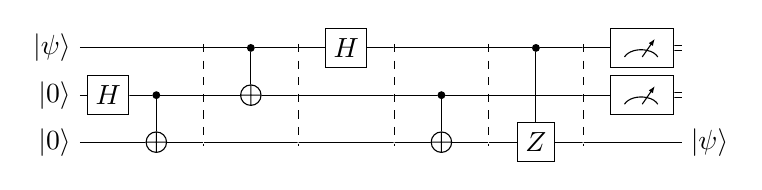
\begin{tikzpicture}
        \begin{yquant}
            qubit {$\ket{\psi}$} q0;
            qubit {$\ket{0}$} q1;
            qubit {$\ket{0}$} q2;
            h q1;
            cnot q2 | q1;
            barrier (-);
            cnot q1 | q0;
            barrier (-);
            h q0;
            barrier (-);
            cnot q2 | q1;
            barrier (-);
            z q2 | q0;
            barrier (-);
            measure q0;
            measure q1;
            output {$\ket{\psi}$} q2;
        \end{yquant}
        \end{tikzpicture}
    \caption{Teleportation using yquant}
    \label{fig:teleportation_yquant}
\end{figure}
\end{document}
